\documentclass[aspectratio=169]{beamer}
\geometry{paperwidth=160mm,paperheight=100mm}
\usepackage{beamerthemesidebar}
\usepackage{hyperref}
\usepackage{color}
\usepackage{multimedia}
\usepackage{colortbl}
\usepackage{amsmath}
\usepackage{empheq}
\usepackage{cancel}
\usepackage{amssymb}
\usepackage{amsfonts}
\usepackage{lipsum}
\usepackage{tcolorbox}
\usepackage{tabularx}
\usepackage{caption}
\usepackage{bm}

\setbeamersize{sidebar width right=0pt}
\setbeamertemplate{footline}[frame number]
%
\definecolor{orange}{RGB}{250,167,12}
\definecolor{yellow}{RGB}{246,250,12}
\definecolor{green}{RGB}{128,238,1}
\definecolor{black}{RGB}{0,0,0}
\definecolor{blue}{RGB}{0,0,255}
\definecolor{red}{RGB}{255,0,0}
\definecolor{sepia}{RGB}{94,38,18}
\newcommand{\ve}[1]{{\rm\bf {#1}}}
\newcommand{\q}[1]{\textcolor{blue}{#1}}
\newcommand{\blue}[1]{\textcolor{blue}{#1}}
\newcommand{\sepia}[1]{\textcolor{sepia}{#1}}
\newcommand{\red}[1]{\textcolor{red}{#1}}
\newcommand{\green}[1]{\textcolor{green}{#1}}
\newcommand{\yellow}[1]{\textcolor{yellow}{#1}}
\newcommand{\orange}[1]{\textcolor{orange}{#1}}
\definecolor{burlywood}{RGB}{255,211,155}
\definecolor{chocolate}{RGB}{255,127,36}
\definecolor{tan}{RGB}{210,180,140}
%
\def\onethird{{\textstyle{1\over3}}}
\def\twothirds{{\textstyle{2\over3}}}
\def\fourthirds{{\textstyle{4\over3}}}
\def\onehalf{{\textstyle{1\over2}}}
\def\threehalfs{{\textstyle{3\over2}}}
%
\newcommand{\pd}{\partial}
\newcommand{\aMLT}{\alpha_{\rm MLT}}
\newcommand{\Fconv}{F_{\rm conv}}
\newcommand{\Frad}{F_{\rm rad}}
\newcommand{\Ftot}{F_{\rm tot}}
\newcommand{\Hp}{H_p}
\newcommand{\prad}{p_{\rm rad}}
\newcommand{\pgas}{p_{\rm gas}}
\newcommand{\TTc}{T_{\rm c}}
\newcommand{\rhoc}{\rho_{\rm c}}
\newcommand{\Teff}{T_{\rm eff}}
\newcommand{\Fstar}{F_\star}
\newcommand{\pstar}{p_\star}
\newcommand{\Pstar}{P_\star}
\newcommand{\Rstar}{R_\star}
\newcommand{\rhostar}{\rho_\star}
\newcommand{\Tstar}{T_\star}
%
\title{Theoretical Astrophysics I: Physics of Sun and Stars\\
Lecture 11: Binary, Variable stars, and Supernovae}
\author{\texorpdfstring{\sepia{Petri K\"{a}pyl\"{a} Ivan Mili\'{c}}\newline\blue{\url{pkapyla, milic@leibniz-kis.de}}}{}}
\institute{Institut f\"ur Sonnenphysik - KIS, Freiburg}
\date{\today}
%
\begin{document}
\frame{\titlepage}


\section{Recap and intro}
%
\frame{
\frametitle{Recap}
\begin{itemize}
\item We have understood the structure (and a bit of evolution of the stars) though the power of 1-D models. 
\item There we have assumed that the stars are isolated, and spherically symmetric.
\item We have also assumed that the processes in them act extremely slowly. 
\item We allowed for some, miniscule oscillations that allowed us to perform helio/astroseismology.
\item In real life, things are much different...
\end{itemize}
}
%
%
\frame{
\frametitle{Departures from ideal approximations}
\begin{minipage}{0.54\linewidth}
\begin{itemize}
\item Stars are not born alone, and they do not evolve alone. 85\% of all the stars are in the binary systems. 
\item Some stars are highly assymetric, either because of fast rotation or strong magnetic fields (or both!)
\item Some exhibit strong, periodic changes, and can change their brightness substantially with period of order of hours or days. 
\item ...explode and completely change their structure (and eject the material in the interstellar space!)
\end{itemize}
\end{minipage}
\begin{minipage}{0.45\linewidth}
\begin{figure}
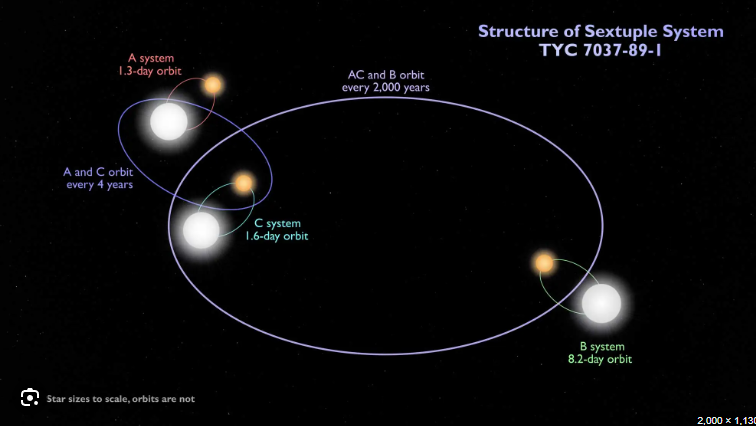
\includegraphics[width=6cm]{figures/multiple_stars.png}
\caption*{Credits: NASA}
\end{figure}
\end{minipage}
}
%
%
\section{Binary Stars}
%
\frame{
\frametitle{Binary stars}
\begin{minipage}{0.54\linewidth}
\begin{itemize}
\item We will focus on systems of two stars, even though there can be more than one. 
\item Note: we are \textbf{not} talking about stellar clusters now.
\item Binary star is a system of two stars that are gravitationally bound to each other.
\item They revolve around the center of the mass of the system.
\end{itemize}
\end{minipage}
\begin{minipage}{0.45\linewidth}
\begin{figure}
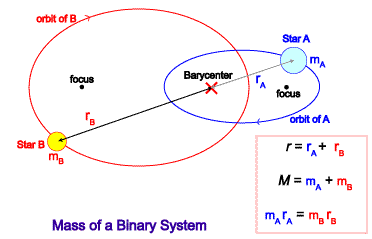
\includegraphics[width=6cm]{figures/binstar.png}
\caption*{Credits: Australia Telescope National Facility}
\end{figure}
\end{minipage}
}
%
\frame{
\frametitle{Visual Binaries}
\begin{minipage}{0.54\linewidth}
\begin{itemize}
\item Binary star is a system of two stars that are gravitationally bound to each other.
\item Sometimes their movement can be detected directly - through the change in the apparent position of the stars on the sky - \textbf{astrometric methods}
\item These stars are often called visual binaries. 
\item To the right we see Sirius, which is in fact a binary star.
\end{itemize}
\end{minipage}
\begin{minipage}{0.45\linewidth}
\begin{figure}
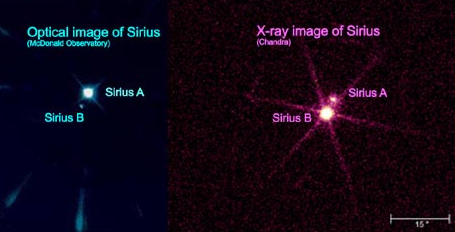
\includegraphics[width=6cm]{figures/sirius.png}
\caption*{Credits: NASA/SAO/CXC/MacDonald Observatory}
\end{figure}
\end{minipage}
}
%
\frame{
\frametitle{Visual Binaries}
\begin{minipage}{0.54\linewidth}
\begin{itemize}
\item We did not immediately discover both. In 1844 Bessel detected that Sirius has a companion, through the change in its proper motion. 
\item In 1915 we observed the spectrum of Sirius B and concluded it is a white dwarf, of the size of the Earth and mass approximately $M_\odot$
\item The orbit of the system is very eccentric ($e=0.6$).
\item Sirius A is an A class star (hehe), with temperature around 10 000\,K and mass equal to 2 $M_\odot$.
\end{itemize}
\end{minipage}
\begin{minipage}{0.45\linewidth}
\begin{figure}
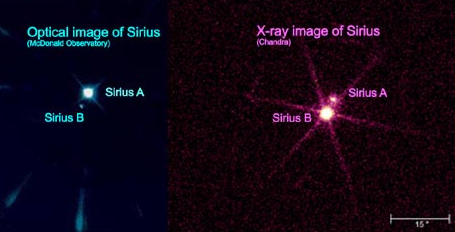
\includegraphics[width=6cm]{figures/sirius.png}
\caption*{Credits: NASA/SAO/CXC/MacDonald Observatory}
\end{figure}
\end{minipage}
}
%
\frame{
\frametitle{Sirius}
\begin{minipage}{0.54\linewidth}
\begin{itemize}
\item Sirius A is an A class star with temperature around 10 000\,K and mass equal to 2 $M_\odot$.
\item Sirius B and concluded is white dwarf, of the size of the Earth and mass approximately $M_\odot$
\item \q{Is there something here that does not fit?}
\end{itemize}
\end{minipage}
\begin{minipage}{0.45\linewidth}
\begin{figure}
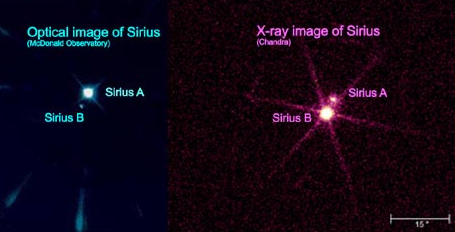
\includegraphics[width=6cm]{figures/sirius.png}
\caption*{Credits: NASA/SAO/CXC/MacDonald Observatory}
\end{figure}
\end{minipage}
}
%
%
\frame{
\frametitle{Sirius}
\begin{minipage}{0.54\linewidth}
\begin{itemize}
\item Sirius A is an A class star with temperature around 10 000\,K and mass equal to 2 $M_\odot$.
\item Sirius B and concluded is white dwarf, of the size of the Earth and mass approximately $M_\odot$
\item \q{Is there something here that does not fit?} - How is less masive star a white dwarf and the more massive one still on the main sequence?
\end{itemize}
\end{minipage}
\begin{minipage}{0.45\linewidth}
\begin{figure}
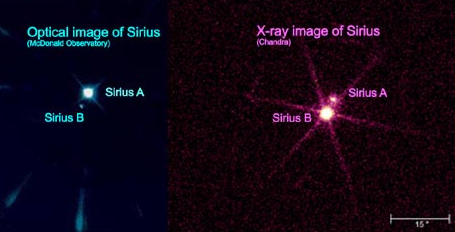
\includegraphics[width=6cm]{figures/sirius.png}
\caption*{Credits: NASA/SAO/CXC/MacDonald Observatory}
\end{figure}
\end{minipage}
}
%
%
\frame{
\frametitle{Sirius}
\begin{minipage}{0.54\linewidth}
\begin{itemize}
\item Sirius A is an A class star with temperature around 10 000\,K and mass equal to 2 $M_\odot$.
\item Sirius B and concluded is white dwarf, of the size of the Earth and mass approximately $M_\odot$
\item \q{Is there something here that does not fit?} - How is less masive star a white dwarf and the more massive one still on the main sequence?
\item Sirius B must have lost a big part of its mass through the evolution.
\item How do we know these stellar masses?
\end{itemize}
\end{minipage}
\begin{minipage}{0.45\linewidth}
\begin{figure}
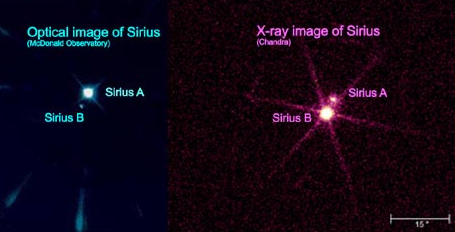
\includegraphics[width=6cm]{figures/sirius.png}
\caption*{Credits: NASA/SAO/CXC/MacDonald Observatory}
\end{figure}
\end{minipage}
}
%
%
\frame{
\frametitle{Visual binaries - mass determination}
\begin{minipage}{0.5\linewidth}
\begin{itemize}
\item Observing systems like this one is crucial for measuring stellar masses.
\item \textbf{First} we measure the period of the system.
\item \textbf{Then} we can use Kepler's third law:
\begin{equation}
\frac{(a1+a2)^3}{T^2} = \frac{G(M_1+ M_2)}{4\pi^2}
\end{equation}
\item To find the mass of the system. Then, we can find individual masses from:
\begin{equation}
M_1 a_1 = M_2 a_2
\end{equation}
\end{itemize}
\end{minipage}
\begin{minipage}{0.49\linewidth}
\begin{figure}
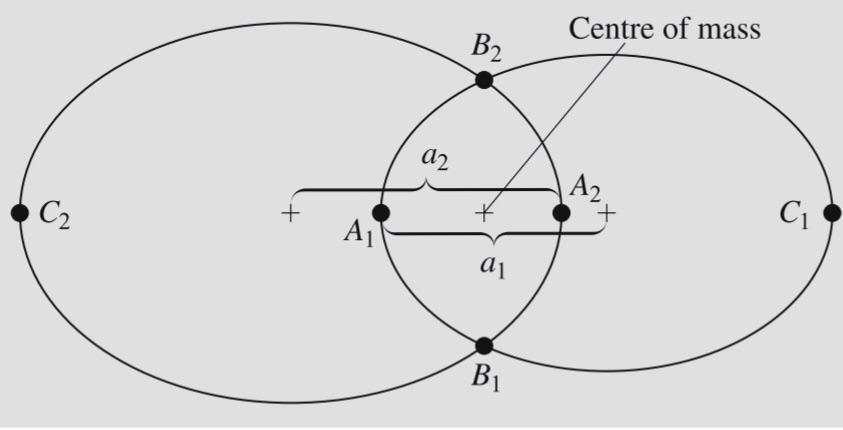
\includegraphics[width=6cm]{figures/orbits.jpg}
\end{figure}
\end{minipage}
}
%
%
\frame{
\frametitle{Visual binaries - mass determination}
\begin{minipage}{0.5\linewidth}
\begin{itemize}
\item \q{What did we have to measure to perform this?}
\end{itemize}
\end{minipage}
\begin{minipage}{0.49\linewidth}
\begin{figure}
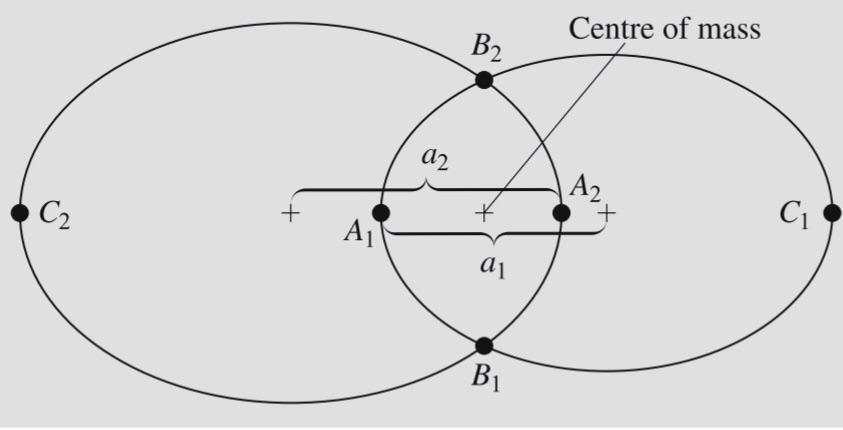
\includegraphics[width=6cm]{figures/orbits.jpg}
\end{figure}
\end{minipage}
}
%
%
\frame{
\frametitle{Visual binaries - mass determination}
\begin{minipage}{0.5\linewidth}
\begin{itemize}
\item \q{What did we have to measure to perform this?}
\item Period of the system 
\item Orbits of both of the stars. 
\item We also needed the orbit to be in the plane of the sky.
\item We need to be a bit fortunate for this to happen!
\item \textbf{But, it allows us to directly measure stellar masses and test our models!}
\end{itemize}
\end{minipage}
\begin{minipage}{0.49\linewidth}
\begin{figure}
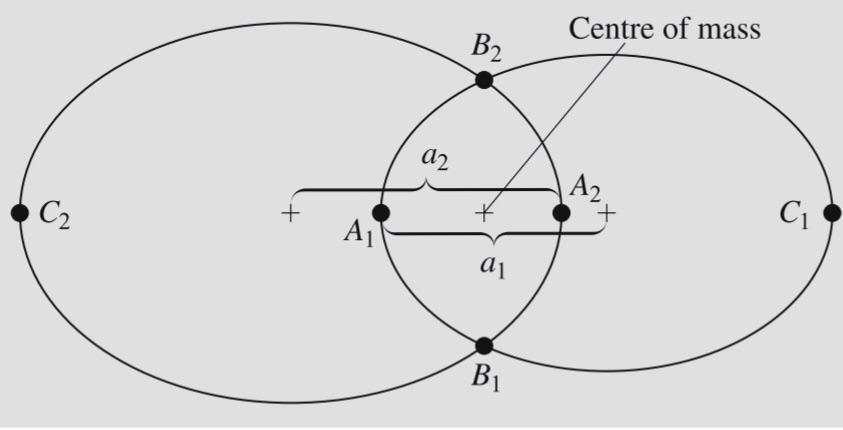
\includegraphics[width=6cm]{figures/orbits.jpg}
\end{figure}
\end{minipage}
}
%
%
\frame{
\frametitle{One more question on Sirius}
\begin{minipage}{0.44\linewidth}
\begin{itemize}
\item \q{How come that Sirius A is brighter in optical wavelengths and Sirius B is brigther in X ray?}
\end{itemize}
\end{minipage}
\begin{minipage}{0.55\linewidth}
\begin{figure}
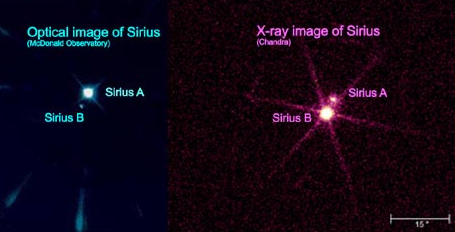
\includegraphics[width=7.5cm]{figures/sirius.png}
\end{figure}
\end{minipage}
}
%
%
\frame{
\frametitle{One more question on Sirius}
\begin{minipage}{0.44\linewidth}
\begin{itemize}
\item \q{How come that Sirius A is brighter in optical wavelengths and Sirius B is brigther in X ray?}
\item $L_\nu \approx B_\nu 4 \pi R^2$
\item Sirius B is smaller but \textbf{much hotter}.
\item Because of non-linearity of Planck function. It can still be brighter in X domain but not in the optical.
\end{itemize}
\end{minipage}
\begin{minipage}{0.55\linewidth}
\begin{figure}
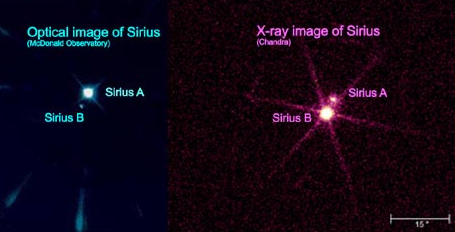
\includegraphics[width=7.5cm]{figures/sirius.png}
\end{figure}
\end{minipage}
}
%
%
\frame{
\frametitle{Spectroscopic binaries}
\begin{minipage}{0.44\linewidth}
\begin{itemize}
\item If we take the spectrum of the binary star, we will see spectral lines shifting to red and blue.
\item This allows us to infer the line-of-sight velocity of these stars: 
\item $v_{los} = \frac{\lambda - \lambda_0}{\lambda_0} c$
\item Today we can measure these velocities down to \textbf{one meter per second}. (E.g. famous HARPS spectrograph).
\end{itemize}
\end{minipage}
\begin{minipage}{0.55\linewidth}
\begin{figure}
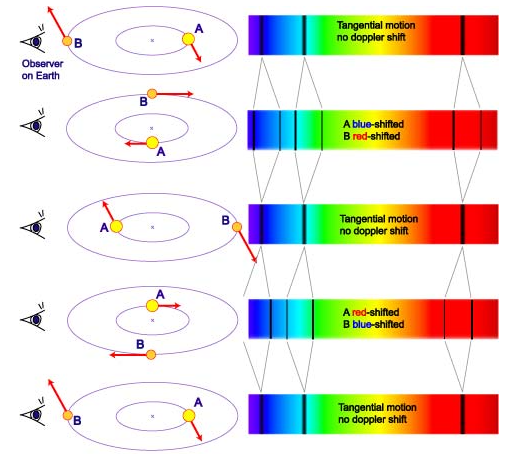
\includegraphics[width=7.5cm]{figures/specb.png}
\end{figure}
\end{minipage}
}
%
\frame{
\frametitle{Spectroscopic binaries and exoplanets}
\begin{minipage}{0.44\linewidth}
\begin{itemize}
\item Sometimes we can only see the spectrum of one component, but we can still detect the shifts. 
\item That still gives us some information about the other component. 
\item The problem is always the inclination of the system w.r.t us.
\item Similar technique is used to detect exoplanets. 
\item \q{What is the relative velocity of the Sun due to influence of the Earth?}
\end{itemize}
\end{minipage}
\begin{minipage}{0.55\linewidth}
\begin{figure}
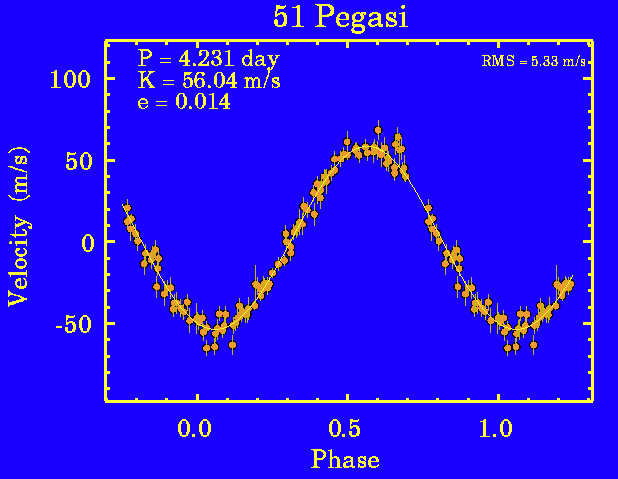
\includegraphics[width=7.5cm]{figures/51p.png}
\end{figure}
\end{minipage}
}
%
%
\frame{
\frametitle{Eclipsing binaries}
\begin{minipage}{0.44\linewidth}
\begin{itemize}
\item If it happens that the orbit of the system coincides with line of sight, we can see the stars eclipse each other.
\item Here we can learn something even if we cannot directly see them separately.
\item \q{What can we learn?}

\end{itemize}
\end{minipage}
\begin{minipage}{0.55\linewidth}
\begin{figure}
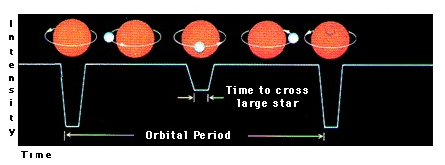
\includegraphics[width=7.5cm]{figures/eb1.png}\\
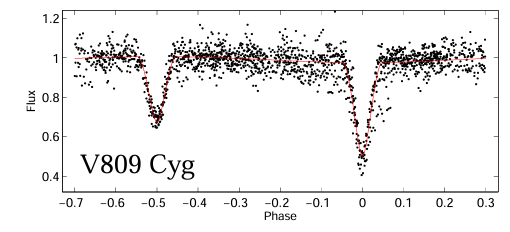
\includegraphics[width=7.5cm]{figures/eb2.png}\\
\end{figure}
\end{minipage}
}
%
\frame{
\frametitle{Eclipsing binaries}
\begin{minipage}{0.44\linewidth}
\begin{itemize}
\item If it happens that the orbit of the system coincides with line of sight, we can see the stars eclipse each other.
\item Here we can learn something even if we cannot directly see them separately.
\item \q{What can we learn?}

\end{itemize}
\end{minipage}
\begin{minipage}{0.55\linewidth}
\begin{figure}
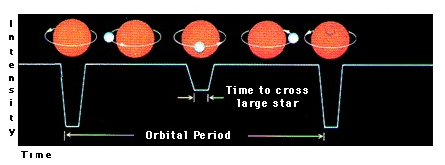
\includegraphics[width=7.5cm]{figures/eb1.png}\\
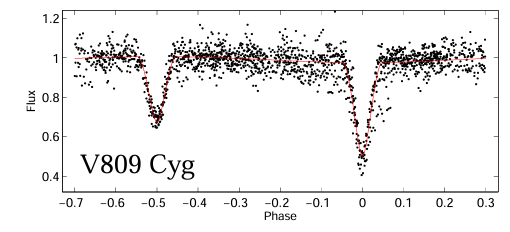
\includegraphics[width=7.5cm]{figures/eb2.png}\\
\end{figure}
\end{minipage}
}
%
%
\frame{
\frametitle{Eclipsing binaries}
\begin{minipage}{0.44\linewidth}
\begin{itemize}
\item Here we can learn something even if we cannot directly see them separately.
\item \q{What can we learn?}
\item The depths of transits and the maximum of brigthness allow us to infer the magnitudes of the components. 
\item Duration of transits $\rightarrow$ sizes of the components. 
\item Shape of the transit and the time difference between primary and secondary transit $\rightarrow$ shape and the orientation of the orbit.
\end{itemize}
\end{minipage}
\begin{minipage}{0.55\linewidth}
\begin{figure}
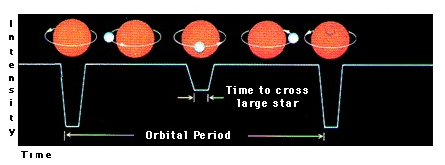
\includegraphics[width=7.5cm]{figures/eb1.png}\\
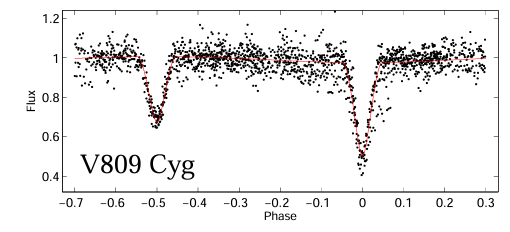
\includegraphics[width=7.5cm]{figures/eb2.png}\\
\end{figure}
\end{minipage}
}
%
%
\frame{
\frametitle{Exoplanet transits}
\begin{minipage}{0.44\linewidth}
\begin{itemize}
\item This is similar to how exoplanet transits work. 
\item Except, of course, planets are much smaller than the stars :-)
\item Several space missions and ground based telescopes have been developed to study exoplanet transits. 
\item For example Kepler space telescope. 
\item What can you conclude from the lightcurve to the right? (\q{Use blackboard})
\end{itemize}
\end{minipage}
\begin{minipage}{0.55\linewidth}
\begin{figure}
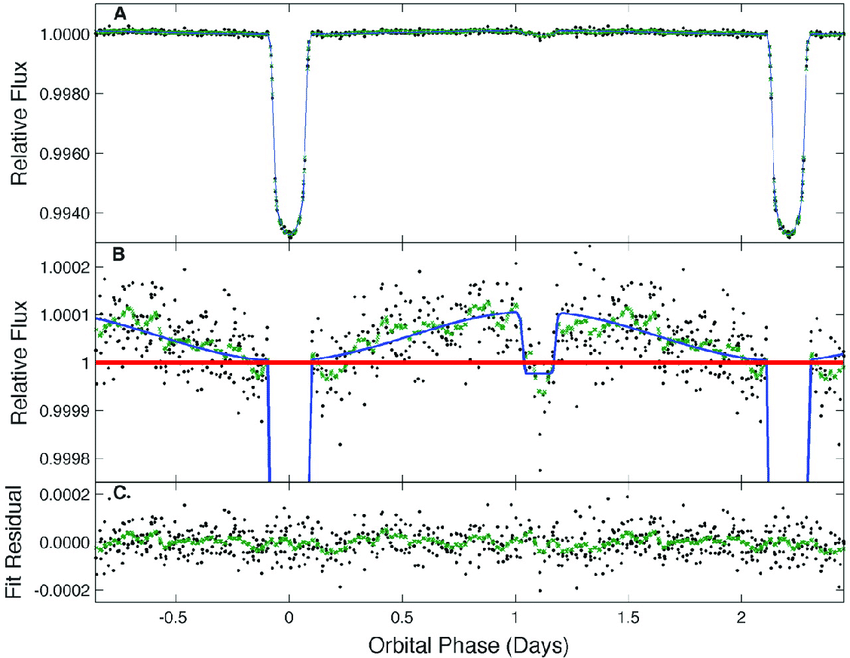
\includegraphics[width=6.5cm]{figures/hatp7b.png}
\caption{Hat P7-b lightcurve. From Borucki et al. 2011}
\end{figure}
\end{minipage}
}
%
%
\frame{
\frametitle{Eclipsing binaries}
\begin{minipage}{0.44\linewidth}
\begin{itemize}
\item \q{Now, what about these lightcurves to the right?}
\end{itemize}
\end{minipage}
\begin{minipage}{0.55\linewidth}
\begin{figure}
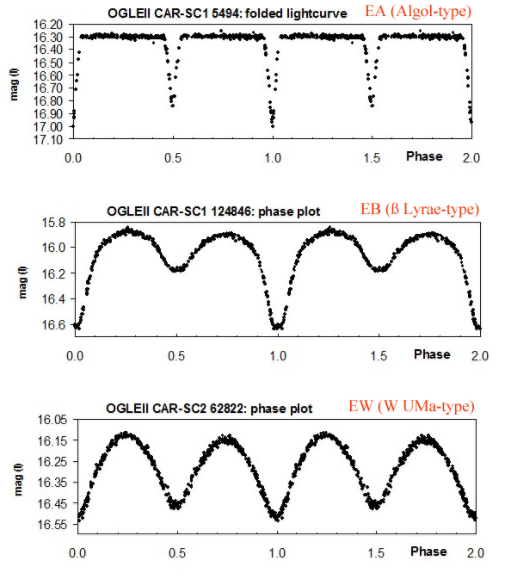
\includegraphics[width=6.5cm]{figures/cebs.png}
\end{figure}
\end{minipage}
}
%
%
\frame{
\frametitle{Close binaries}
\begin{minipage}{0.44\linewidth}
\begin{itemize}
\item \q{Now, what about this lightcurve to the right?}
\item Close binary systems are binary stars where the components are so close to each other that they physically pertub each other's shape. 
\item The stars are sometimes in contact - with the mass flow from one to the other. 
\item Obviously, these stars are not perfect, 1D spherically symmetric!
\end{itemize}
\end{minipage}
\begin{minipage}{0.55\linewidth}
\begin{figure}
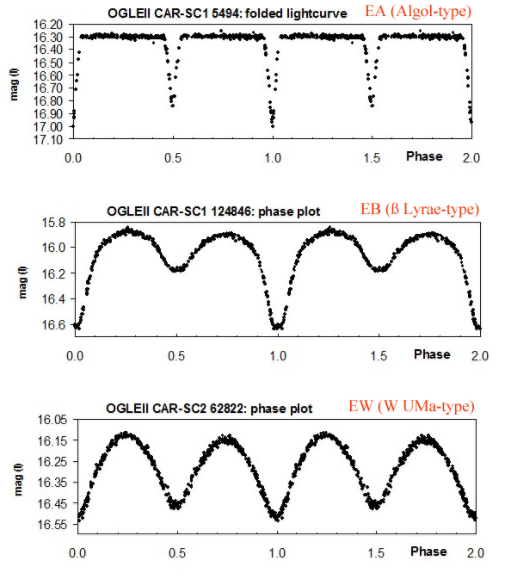
\includegraphics[width=6.5cm]{figures/cebs.png}
\end{figure}
\end{minipage}
}
%
%
\frame{
\frametitle{Close binaries}
\begin{minipage}{0.44\linewidth}
\begin{itemize}
\item Modeling and understand curves of close (interacting) binaries requires detailed understanding of their shapes and corresponding distortions of their atmospheres. 
\item One often introduces bright or dark spots on the stellar surface. 
\item Inferring the properties of these objects is done through the light curve fitting where we fit the model of the system to the lightcurves (often recorded in different filters).
\item If you want to know more about this, sign up for WS 2024 (``Remote sensing'' course).
\end{itemize}
\end{minipage}
\begin{minipage}{0.55\linewidth}
\begin{figure}
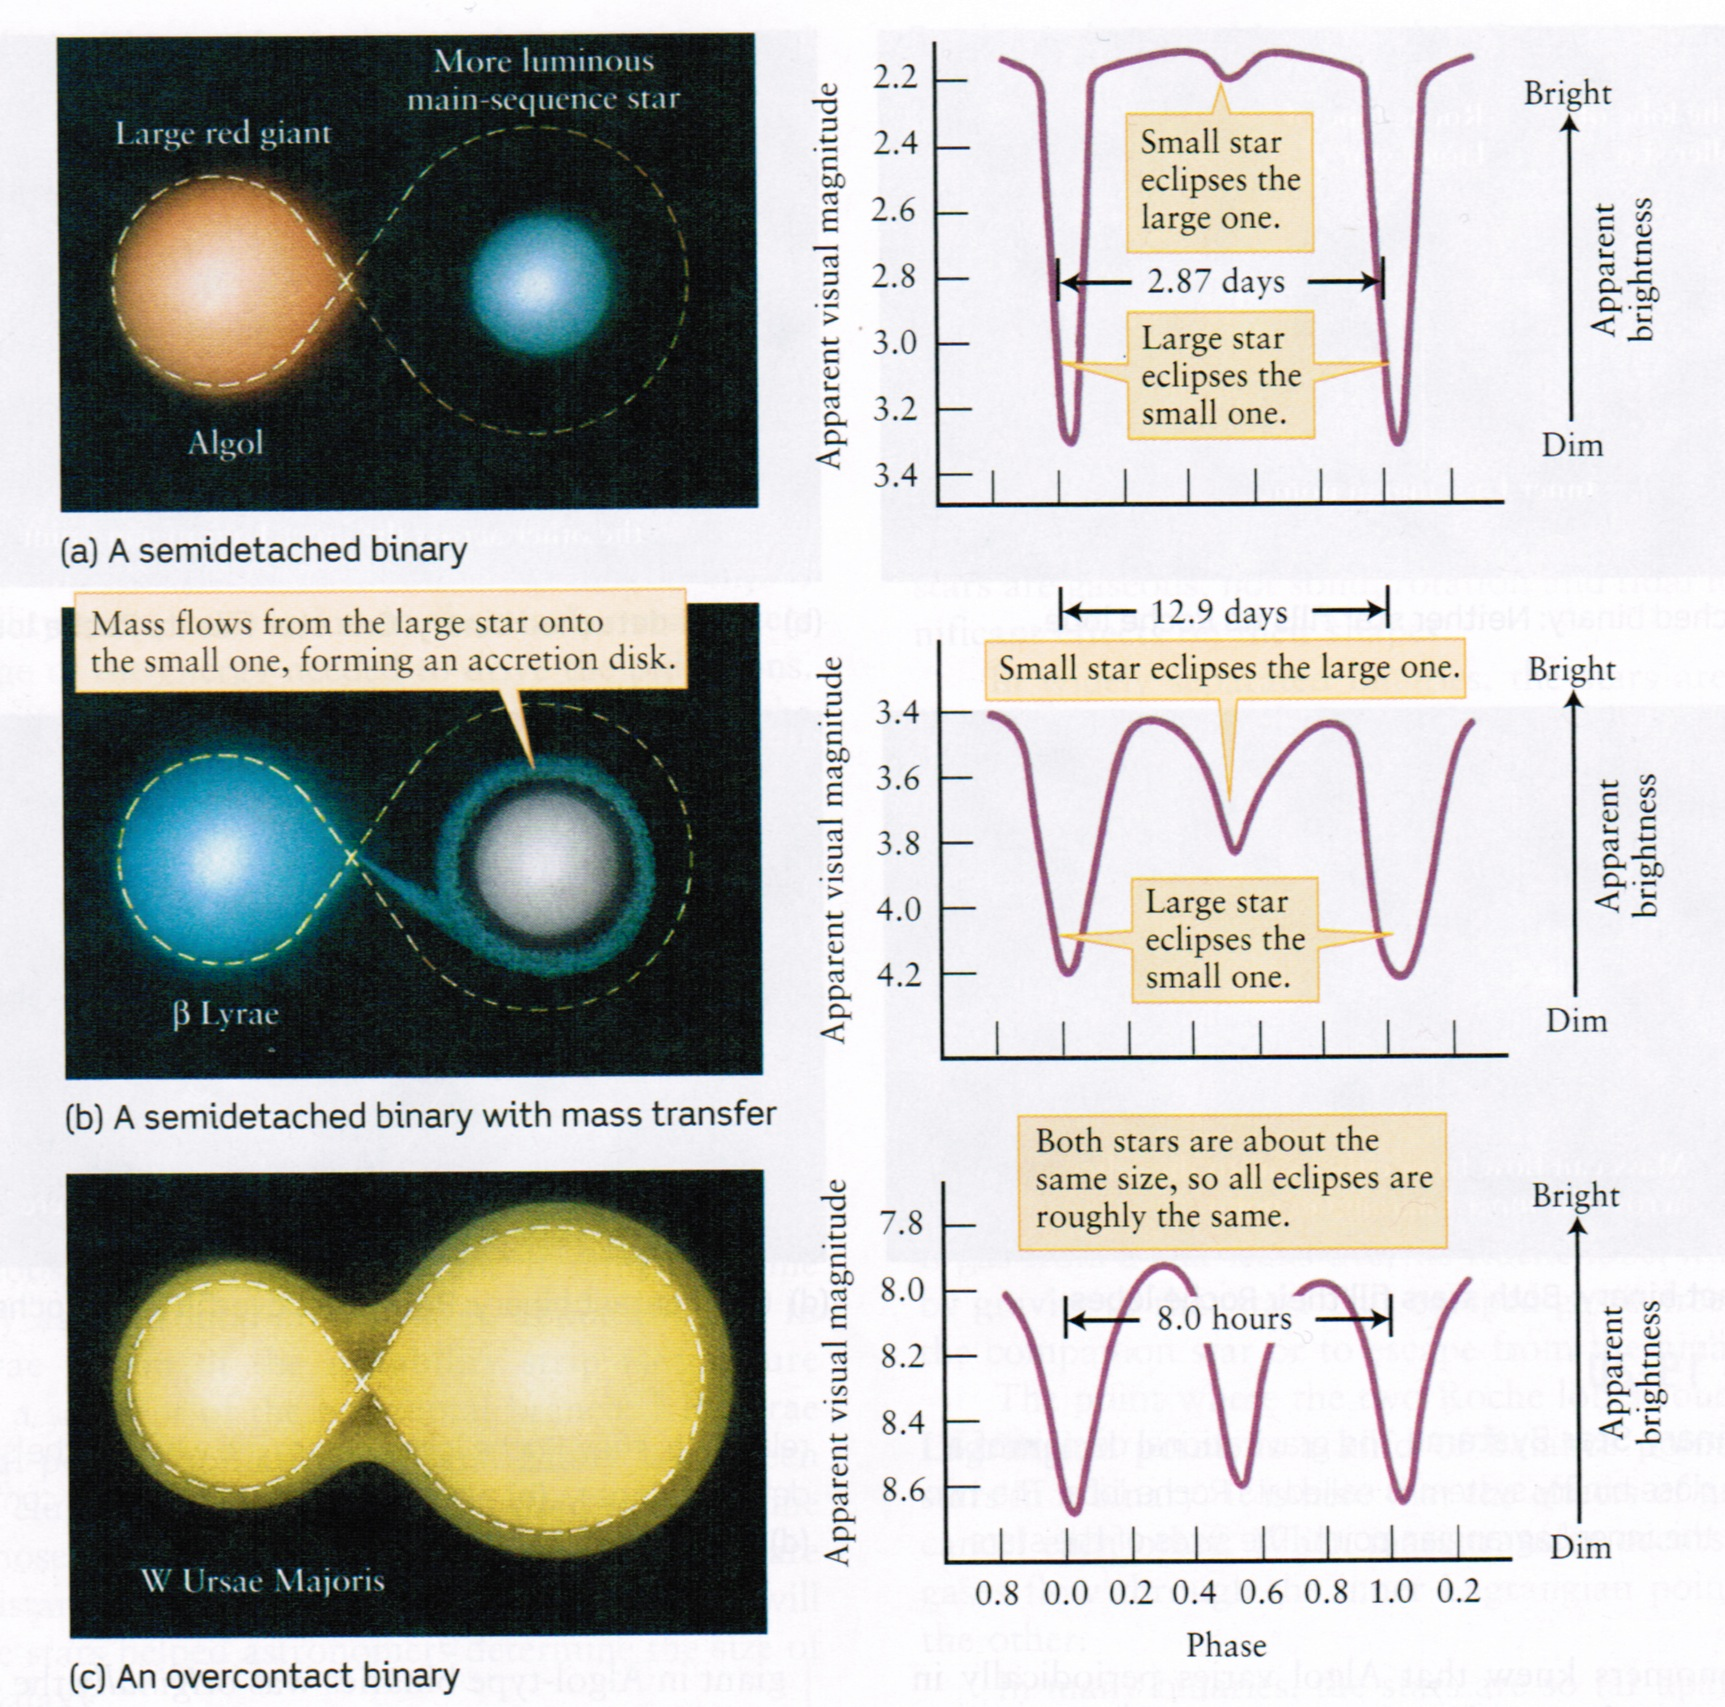
\includegraphics[width=6.5cm]{figures/feb.jpeg}
\end{figure}
\end{minipage}
}
%
%
\frame{
\frametitle{Close binaries}
\begin{minipage}{0.44\linewidth}
\begin{itemize}
\item Sometimes there is even an accretion disk around one of the components.
\item The accretion disk itself can heat up significantly due to ``friction'' and reach very high temperatures, thus emitting substantially in X-domain.
\item If you want to know more about this, sign up for WS 2024 (``Remote sensing'' course).
\end{itemize}
\end{minipage}
\begin{minipage}{0.55\linewidth}
\begin{figure}
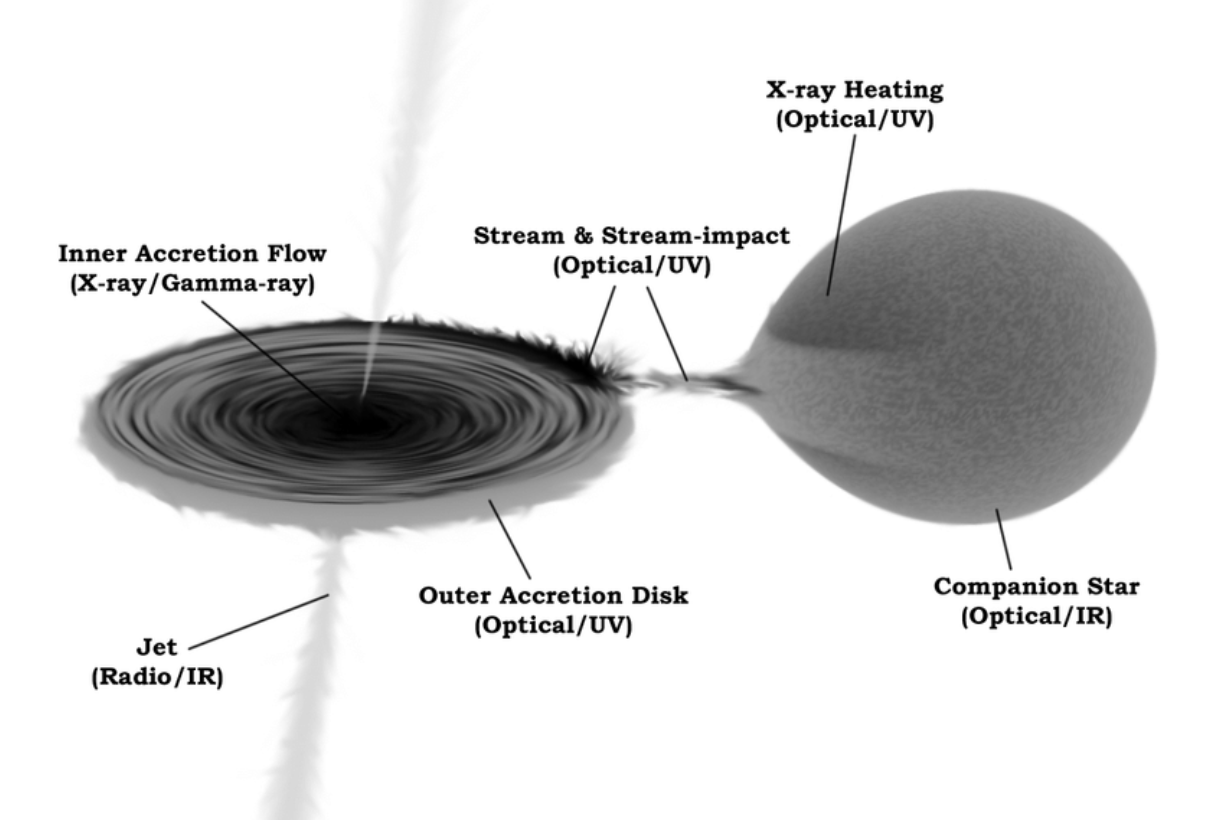
\includegraphics[width=6.5cm]{figures/xray.png}
\end{figure}
\end{minipage}
}
%
\frame{
\frametitle{How come we are not in a binary star system?}
\begin{minipage}{0.5\linewidth}
\begin{itemize}
\item If 85\% of the stars are in the binary systems, how come we are living in the system with a single star? 
\end{itemize}
\end{minipage}
\begin{minipage}{0.49\linewidth}
\begin{figure}
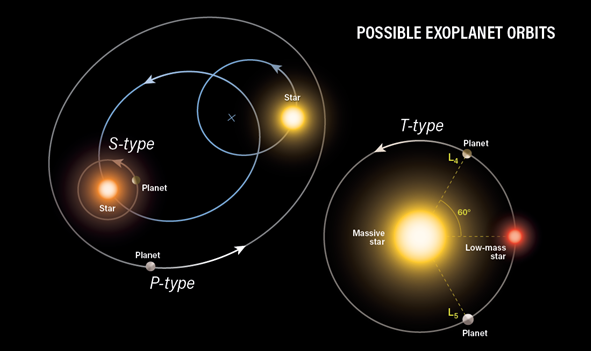
\includegraphics[width=7.5cm]{figures/planetbinary.png}
\caption*{Credits: ESA}
\end{figure}
\end{minipage}
}
%
%
\frame{
\frametitle{How come we are not in a binary star system?}
\begin{minipage}{0.5\linewidth}
\begin{itemize}
\item \q{If 85\% of the stars are in the binary systems, how come we are living in the system with a single star?}
\item In multiple star system the planet would suffer large variations of irradiance.
\item These would make temperature very unstable (can you estimate?).
\item Which would, probably, severly hamper chances of developing life. 
\end{itemize}
\end{minipage}
\begin{minipage}{0.49\linewidth}
\begin{figure}
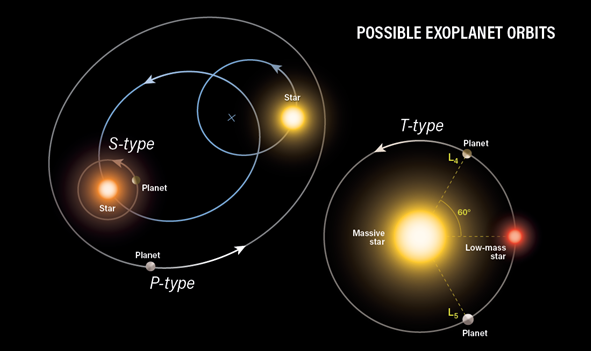
\includegraphics[width=7.5cm]{figures/planetbinary.png}
\caption*{Credits: ESA}
\end{figure}
\end{minipage}
}
%
%
\frame{
\frametitle{Stellar evolution in close binary systems}
\begin{minipage}{0.50\linewidth}
\begin{itemize}
\item When the star evolves and expands (e.g. red giant phase), the Roche lobe will overflow. 
\item The material will flow onto the other (less massive) star, accelerating her evolution. 
\item The whole story can happen again... Second component overflows, dumping material onto the white dwarf.
\item Sometimes this material ignites in the TN reactions, creating a \textbf{Type Ia Supernova!}.
\end{itemize}
\end{minipage}
\begin{minipage}{0.49\linewidth}
\begin{figure}
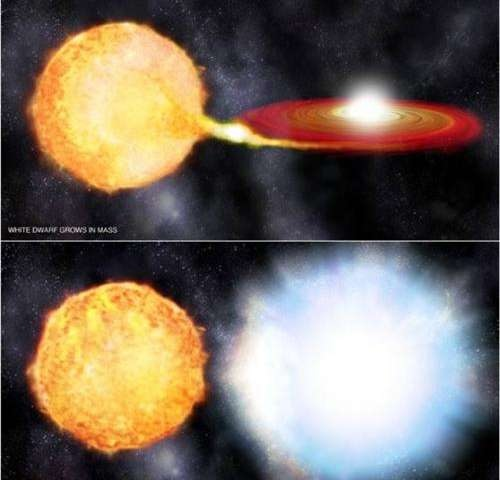
\includegraphics[width=6.5cm]{figures/type1.jpg}
\caption*{Credits: NASA/CXC/M. Weiss}
\end{figure}
\end{minipage}
}
%
%
\frame{
\frametitle{Supernovae classification}
\begin{figure}
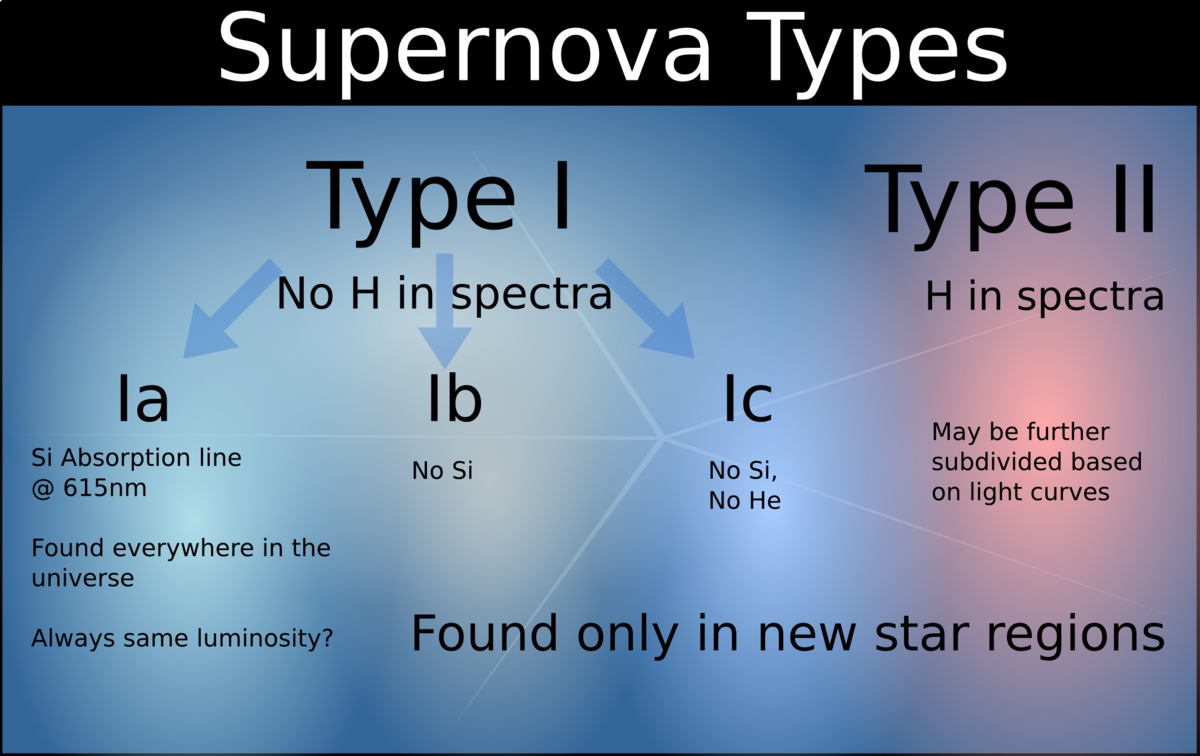
\includegraphics[width=11cm]{figures/snc.png}
\caption*{Supernovae classification. Credits:Stanford University}
\end{figure}
}
%
%
\frame{
\frametitle{Core-collapse supernovae}
\begin{figure}
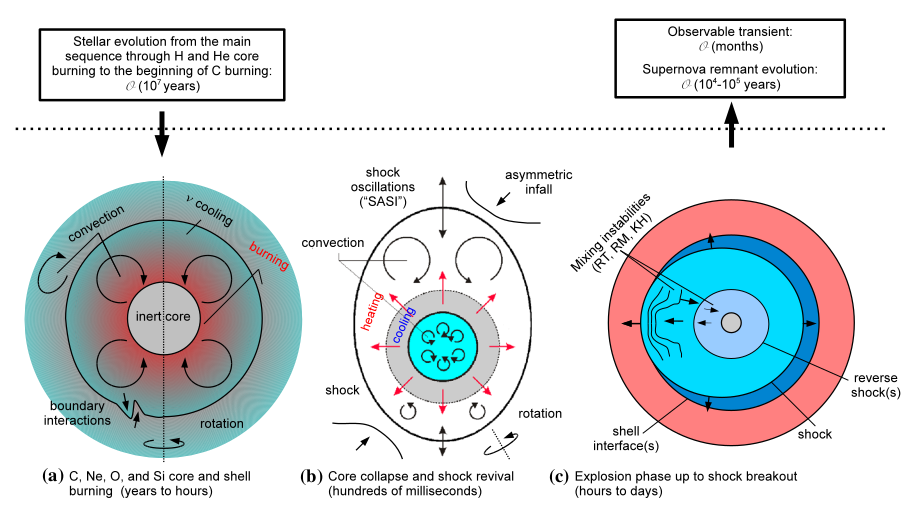
\includegraphics[width=11cm]{figures/ccsne.png}
\caption*{Hydrodynamics of a core-collapse supernova. Credits: M\"{u}ller, 2020}
\end{figure}
}
%
%
\frame{
\frametitle{SNe type 1a - Standard candles}
\begin{minipage}{0.50\linewidth}
\begin{itemize}
\item \textbf{Standard candle} - an object whose absolute magnitude (luminosity) we know with a high accuracy.
\item SNe type1a are standard candles because they ignite when an exact mass is reached. 
\item They are also bright - making them suitable for distance measurement. 
\item There is still a number of uncertainties (chemical composition, interstellar absorption...)
\end{itemize}
\end{minipage}
\begin{minipage}{0.49\linewidth}
\begin{figure}
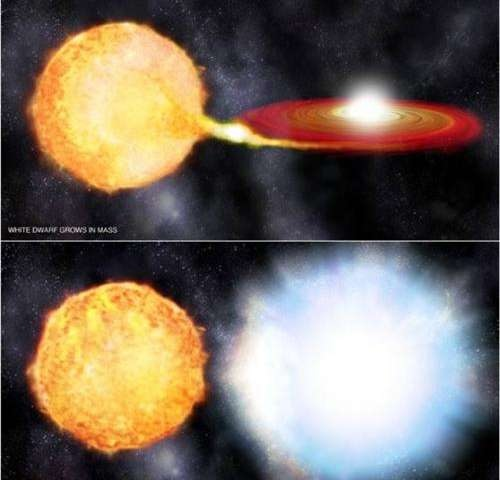
\includegraphics[width=6.5cm]{figures/type1.jpg}
\caption*{Credits: NASA/CXC/M. Weiss}
\end{figure}
\end{minipage}
}
%
%
\frame{
\frametitle{SNe type 1a - Standard candles}
\begin{minipage}{0.50\linewidth}
\begin{itemize}
\item \textbf{Standard candle} - an object whose absolute magnitude (luminosity) we know with a high accuracy.
\begin{equation}
m = M - 5 + 5\log d
\end{equation}
\item By observing a swath of supernovae, supernova cosmology project managed to map the geometry of spacetime and infer that the universe expands with some acceleration.
\item Nobel prize 2011.
\end{itemize}
\end{minipage}
\begin{minipage}{0.49\linewidth}
\begin{figure}
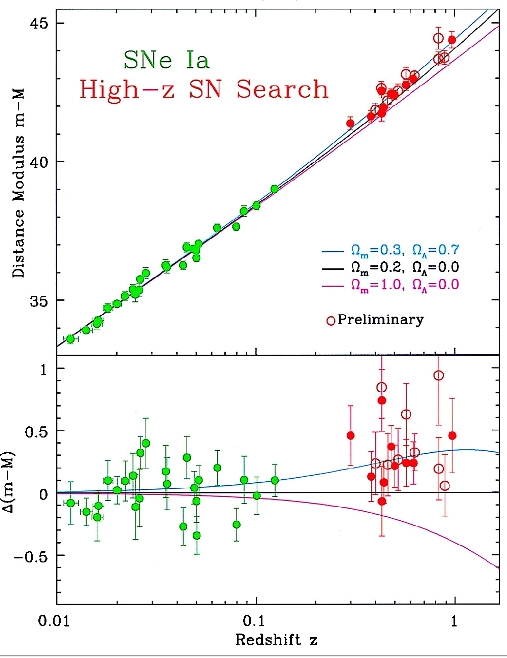
\includegraphics[width=6.5cm]{figures/snep.png}
\caption*{Hubble diagram from supernova cosmology project. Credits: Kirschner, 1998}
\end{figure}
\end{minipage}
}
%
%
\frame{
\frametitle{How did this story start?}
\begin{minipage}{0.50\linewidth}
\begin{itemize}
\item Edwin Hubble observed variable stars in other ``nebulae'' and measured distance to them. 
\item He also used measurements of radial velocity made by Vesto Slipher to construct a simple Hubble diagram. 
\item The relationship between the distance and velocity implied that universe is expanding. 
\item This is consistent with a solution of Einstein's equation. 
\end{itemize}
\end{minipage}
\begin{minipage}{0.49\linewidth}
\begin{figure}
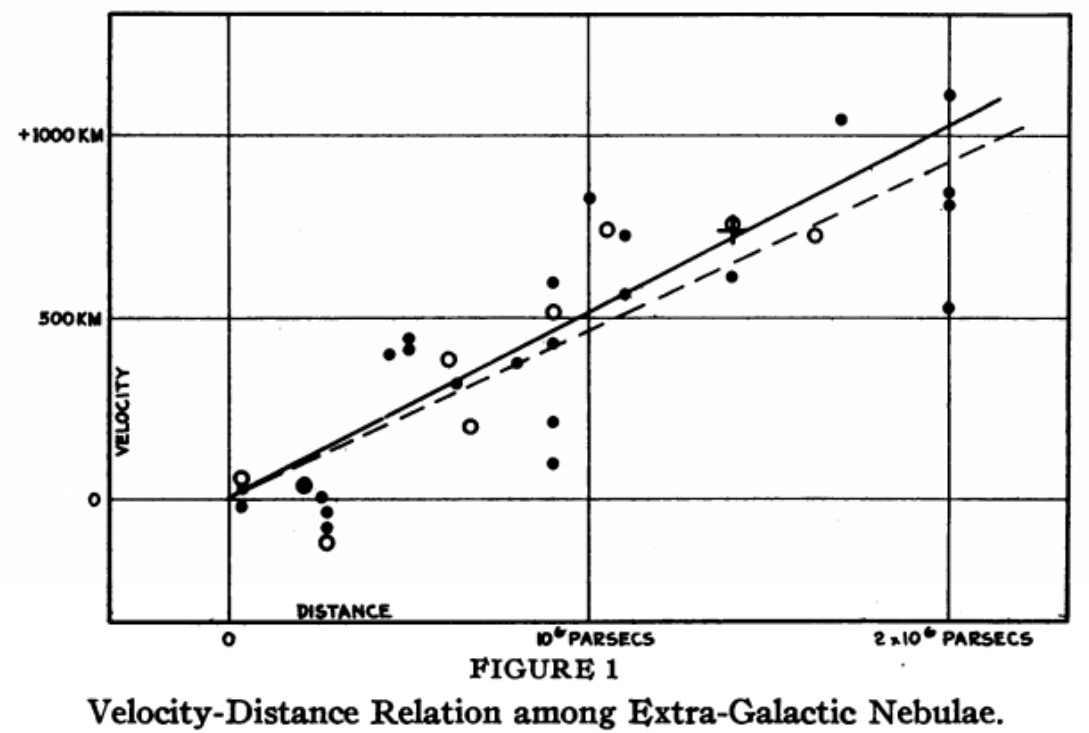
\includegraphics[width=6.5cm]{figures/hubbled.png}
\caption*{Hubble diagram from supernova cosmology project. Credits: Kirschner, 1998}
\end{figure}
\end{minipage}
}
%
%
\frame{
\frametitle{}
\begin{figure}
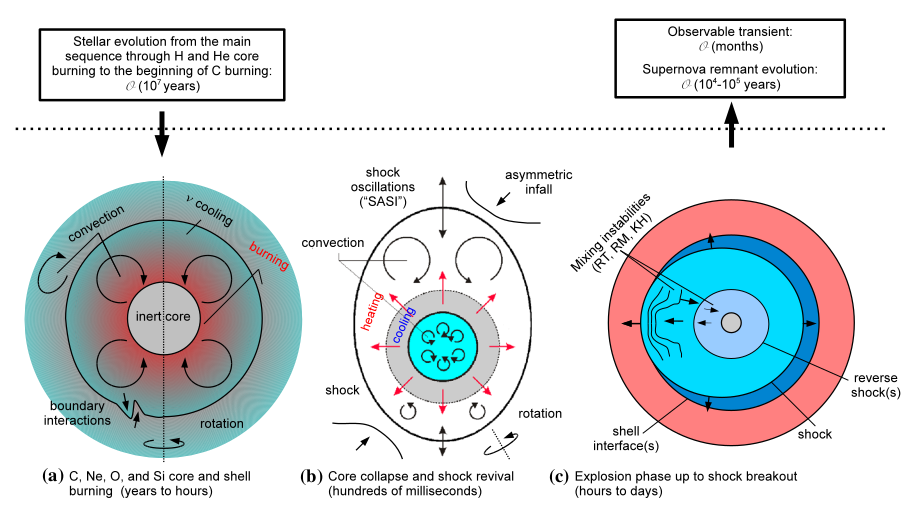
\includegraphics[width=11cm]{figures/ccsne.png}
\caption*{Hydrodynamics of a core-collapse supernova. Credits: M\"{u}ller, 2020}
\end{figure}
}
%
\end{document}
% 

